% $Header: /Users/joseph/Documents/LaTeX/beamer/solutions/conference-talks/conference-ornate-20min.en.tex,v 90e850259b8b 2007/01/28 20:48:30 tantau $

\documentclass[xcolor={usenames,dvipsnames}]{beamer}

% This file is a solution template for:

% - Talk at a conference/colloquium.
% - Talk length is about 20min.
% - Style is ornate.



% Copyright 2004 by Till Tantau <tantau@users.sourceforge.net>.
%
% In principle, this file can be redistributed and/or modified under
% the terms of the GNU Public License, version 2.
%
% However, this file is supposed to be a template to be modified
% for your own needs. For this reason, if you use this file as a
% template and not specifically distribute it as part of a another
% package/program, I grant the extra permission to freely copy and
% modify this file as you see fit and even to delete this copyright
% notice. 


\mode<presentation>
{
  \usetheme{AnnArbor}
  % or ...

  \setbeamercovered{transparent}
  % or whatever (possibly just delete it)
 }

\usepackage[percent]{overpic}

\usepackage[english]{babel}
% or whatever

\usepackage[latin1]{inputenc}
% or whatever

\usepackage{times}
\usepackage[T1]{fontenc}
% Or whatever. Note that the encoding and the font should match. If T1
% does not look nice, try deleting the line with the fontenc.
%particles
\newcommand{\jpsi}{\rm J/$\psi$}
\newcommand{\psip}{$\psi^\prime$}
\newcommand{\jpsiDY}{\rm J/$\psi$\,/\,DY}
\newcommand{\chic}{$\chi_{\rm c}$}
\newcommand{\pip}{$\pi^{+}$}
\newcommand{\pim}{$\pi^{-}$}
\newcommand{\pizero}{$\pi^{0}$}
\newcommand{\kap}{K$^{+}$}
\newcommand{\kam}{K$^{-}$}
\newcommand{\pbar}{$\rm\overline{p}$}
\newcommand{\ccbar}{\ensuremath{\mathrm{c\overline{c}}}}
\newcommand{\bbbar}{\ensuremath{\mathrm{b\overline{b}}}}
\newcommand{\Dzero}{\ensuremath{\mathrm{D^{0}}}}
\newcommand{\Dzerobar}{\ensuremath{\mathrm{\overline{D}^{0}}}}
\newcommand{\Dpm}{\ensuremath{\mathrm{D^{\pm}}}}
\newcommand{\Ds}{\ensuremath{\mathrm{D_{s}^{\pm}}}}
\newcommand{\Dstar}{\ensuremath{\mathrm{D^{*\pm}}}}

%collision systems
\newcommand{\pp}{pp}
\newcommand{\pPb}{p--Pb}
\newcommand{\PbPb}{Pb--Pb}

%detectors
\newcommand{\ezdc}{$E_{\rm ZDC}$}

%units
\newcommand{\GeVc}{GeV/$c$}
\newcommand{\GeVcsq}{GeV/$c^2$}

%others
\newcommand{\degree}{$^{\rm o}$}
\newcommand{\s}{\ensuremath{\sqrt{s}}}
\newcommand{\snn}{\ensuremath{\sqrt{s_{\rm NN}}}}
\newcommand{\y}{\ensuremath{y}}
\newcommand{\pt}{\ensuremath{p_{\rm T}}}
\newcommand{\dedx}{d$E$/d$x$}
\newcommand{\dndy}{d$N$/d$y$}
\newcommand{\dndydpt}{${\rm d}^2N/({\rm d}y {\rm d}p_{\rm t})$}
\newcommand{\zpar}{\ensuremath{z_{||}}}
\newcommand{\zpargen}{\ensuremath{z_{||}^{\mathrm{part}}}}
\newcommand{\zpardet}{\ensuremath{z_{||}^{\mathrm{det}}}}
\newcommand{\ptchjet}{\ensuremath{p_{\mathrm{T,ch\, jet}}}}
\newcommand{\ptjet}{\ensuremath{p_{\mathrm{T,jet}}}}
\newcommand{\ptchjetgen}{\ensuremath{p_{\mathrm{T,ch\,jet}}^{\mathrm{part}}}}
\newcommand{\ptchjetdet}{\ensuremath{p_{\mathrm{T,ch\,jet}}^{\mathrm{det}}}}
\newcommand{\ptd}{\ensuremath{p_{\mathrm{T,D}}}}
\newcommand{\ptdgen}{\ensuremath{p_{\mathrm{T,D}}^{\mathrm{part}}}}
\newcommand{\ptddet}{\ensuremath{p_{\mathrm{T,D}}^{\mathrm{det}}}}
\newcommand{\antikt}{anti-\ensuremath{k_{\mathrm{T}}}}
\newcommand{\Antikt}{Anti-\ensuremath{k_{\mathrm{T}}}}
\newcommand{\kt}{\ensuremath{k_{\mathrm{T}}}}
\newcommand{\pthard}{\ensuremath{p_{\mathrm{T,hard}}}}

\title[D-tagged jets in pp collisions at 7 TeV] % (optional, use only with long paper titles)
{D-meson tagged jets in pp collisions at 7 TeV}

\author[Salvatore Aiola]% (optional, use only with lots of authors)
{Salvatore Aiola}
% - Give the names in the same order as the appear in the paper.
% - Use the \inst{?} command only if the authors have different
%   affiliation.

\institute[Yale University] % (optional, but mostly needed)
{Yale University}

\date[PWG-JE - Sept. 9th, 2016] % (optional, should be abbreviation of conference name)
{PWG-JE \\
September 9th, 2016}
% - Either use conference name or its abbreviation.
% - Not really informative to the audience, more for people (including
%   yourself) who are reading the slides online

\subject{High-Energy Physics}
% This is only inserted into the PDF information catalog. Can be left
% out. 



% If you have a file called "university-logo-filename.xxx", where xxx
% is a graphic format that can be processed by latex or pdflatex,
% resp., then you can add a logo as follows:

% \pgfdeclareimage[height=0.5cm]{university-logo}{university-logo-filename}
% \logo{\pgfuseimage{university-logo}}


% If you wish to uncover everything in a step-wise fashion, uncomment
% the following command: 

%\beamerdefaultoverlayspecification{<+->}


\begin{document}

\begin{frame}
  \titlepage
\end{frame}


% Structuring a talk is a difficult task and the following structure
% may not be suitable. Here are some rules that apply for this
% solution: 

% - Exactly two or three sections (other than the summary).
% - At *most* three subsections per section.
% - Talk about 30s to 2min per frame. So there should be between about
%   15 and 30 frames, all told.

% - A conference audience is likely to know very little of what you
%   are going to talk about. So *simplify*!
% - In a 20min talk, getting the main ideas across is hard
%   enough. Leave out details, even if it means being less precise than
%   you think necessary.
% - If you omit details that are vital to the proof/implementation,
%   just say so once. Everybody will be happy with that.

\section{Outline}
\begin{frame}{Updates}
\begin{itemize}
\item Implementation of two additional methods for D-Tagged Jet signal extraction
\begin{itemize}
\item \textcolor{BrickRed}{\textbf{Side-Band}} background subtraction
\item \textcolor{ForestGreen}{\textbf{Like-Sign}} background subtraction
\end{itemize}
\item Motivation
\begin{itemize}
\item Cross-check for \textcolor{NavyBlue}{\textbf{invariant mass fit}} method for possible biases
\item S-B and L-S can be more stable compared to the invariant mass fit for low signal/background (but with larger statistical uncertainties)
\end{itemize}
\item These slides are based on my HQ16 talk
\end{itemize}
\end{frame}

\section{Analysis Overview}
\begin{frame}{D-meson jet tagging}
\begin{enumerate}
\item For each \Dzero\ meson candidate that passes \alert{PID} and \alert{topological} cuts utilize \antikt\ \alert{jet finding}\\ (\pt\ recombination scheme)
\begin{itemize}
\item \Dzero\ candidate 4-momentum
\item all other reconstructed tracks
\item exclude candidate daughters
\end{itemize}
\item Combinatorial background from random $\mathrm{K}\pi$ pairs 
\begin{itemize}
\item[$\rightarrow$] \alert{invariant mass analysis} to extract signal
\end{itemize}
\end{enumerate}
\bigskip
\textbf{\alert{\Dzero(\Dzerobar) meson}}
\begin{itemize}
\item $M=1.865$~\GeVcsq, $c\tau=123\,\mu\mathrm{m}$ 
\item Decay: \Dzero$\rightarrow\mathrm{K}^+\pi^-$ and c.c. with ${\rm BR}=3.88\%$
\end{itemize}
\end{frame}


\section{Signal Extraction}
\subsection{D-tagged jet signal extraction}
\begin{frame}{Signal extraction}

{\Large
\textbf{\alert{Three methods}}
\begin{enumerate}
\bigskip
\item \textcolor{BrickRed}{Side-Band (S-B) background subtraction}
\medskip
\item \textcolor{ForestGreen}{Like-Sign (L-S) background subtraction}
\medskip
\item \textcolor{NavyBlue}{Invariant Mass Fit in bins of \ptchjet}
\end{enumerate}
}
\end{frame}

\begin{frame}[t]{Signal extraction: S-B method}
\begin{columns}[T]
\column{.50\textwidth}
\begin{overpic}[width=\textwidth, trim=0 0 0 50, clip]{img/HQ16_Simulation_InvMassSB}
\end{overpic}
\column{.50\textwidth}
\textbf{\textcolor{BrickRed}{Method 1: Side-Band (S-B)}}
\begin{enumerate}
\item Fill D-meson invariant mass distributions in bins of \alert{\ptd}
\item $N(\ptchjet, \ptd)$ distributions in\\
\medskip
\textcolor{NavyBlue}{\textbf{Peak Area}
{\scriptsize $|M_{\rm K\pi} - M_{\rm fit}| <2\sigma$}\\ 
\smallskip
$N_{\rm sig+bkg} (\ptchjet, \ptd)$}\\
\medskip
\textcolor{BrickRed}{\textbf{Side Bands}
{\scriptsize $8\sigma <|M_{\rm K\pi} - M_{\rm fit}| < 4\sigma$}\\ 
\smallskip
$N_{\rm bkg, SB} (\ptchjet, \ptd)$}
\end{enumerate}
\end{columns}
\begin{enumerate}
\setcounter{enumi}{2}
\item Apply \textcolor{VioletRed}{efficiency correction} and \textcolor{YellowOrange}{integrate in \ptd}
{\small $$N_{\rm signal} (\ptchjet)=\textcolor{YellowOrange}{\sum_{\ptd}} \textcolor{VioletRed}{\frac{1}{\epsilon(\ptd)}} [\textcolor{NavyBlue}{N_{\rm sig+bkg}(\ptchjet, \ptd)} - \textcolor{BrickRed}{N_{\rm bkg,SB}(\ptchjet, \ptd)}]$$}
\end{enumerate}
\end{frame}

\begin{frame}[t]{Signal extraction: L-S method}
\begin{columns}[T]
\column{.50\textwidth}
\begin{overpic}[width=\textwidth, trim=0 0 0 50, clip]{img/HQ16_Simulation_InvMassSB}
\end{overpic}
\column{.50\textwidth}
\textbf{\textcolor{ForestGreen}{Method 2: Like-Sign (L-S)}}
\begin{enumerate}
\item Fill D-meson invariant mass distributions in bins of \alert{\ptd}
\item $N(\ptchjet, \ptd)$ distributions in\\
\medskip
\textcolor{NavyBlue}{\textbf{U-S peak area} {\footnotesize $|M_{\rm K\pi} - M_{\rm fit}| <2\sigma$}\\ 
\smallskip
{\small $N_{\rm sig+bkg} (\ptchjet, \ptd)$}}\\
\medskip
\textcolor{ForestGreen}{\textbf{L-S peak area} {\footnotesize $|M_{\rm K\pi} - M_{\rm fit}| <2\sigma$}\\ 
\smallskip
{\small $N_{\rm bkg, LS} (\ptchjet, \ptd)$}}
\end{enumerate}
\end{columns}
\begin{enumerate}
\setcounter{enumi}{2}
\item Apply \textcolor{VioletRed}{efficiency correction} and \textcolor{YellowOrange}{integrate in \ptd}
{\small $$N_{\rm signal} (\ptchjet)=\textcolor{YellowOrange}{\sum_{\ptd}} \textcolor{VioletRed}{\frac{1}{\epsilon(\ptd)}} [\textcolor{NavyBlue}{N_{\rm sig+bkg}(\ptchjet, \ptd)} - \textcolor{ForestGreen}{N_{\rm bkg,LS}(\ptchjet, \ptd)}]$$}
\end{enumerate}
\end{frame}

\begin{frame}[t]{Signal extraction: invariant mass fit}
\begin{columns}[T]
\column{.5\textwidth}
\begin{overpic}[width=\textwidth, trim=190 0 190 175, clip]{img/D0_JetPtBins_PtD_20}
\end{overpic}
\column{.5\textwidth}
\textbf{\textcolor{NavyBlue}{Method 3: invariant mass fit}}
\begin{enumerate}
\item Fill D-meson invariant mass distributions in bins of \alert{\ptchjet}
\item \textbf{Fit invariant mass distributions} with a \\ Gaussian (\textcolor{NavyBlue}{signal}) + exponential (\textcolor{BrickRed}{background})
\item Extract $N_{\rm signal} (\ptchjet)$ from fit parameters
\end{enumerate}
\end{columns}
\begin{itemize}
\item The correction for the D-tagged jet reconstruction efficiency must be applied as a weight when filling the invariant mass plots
\end{itemize}
\end{frame}

\subsection{Method comparison}
\begin{frame}{Method comparison}
\begin{columns}
\column{.55\textwidth}
\begin{overpic}[width=\textwidth, trim=0 0 50 0, clip]{img/HQ16_Simulation_MethodComparison}
\end{overpic}
\column{.45\textwidth}
\begin{itemize}
\item The \textbf{\textcolor{NavyBlue}{invariant mass fit}}, \textbf{\textcolor{BrickRed}{Side-Band}} 
and \textbf{\textcolor{ForestGreen}{Like-Sign}} methods \textbf{agree well} with the MC truth within their statistical uncertainties
\medskip
\item There is a chance of a (small) systematic bias (all points seem to be above unity) $\rightarrow$ to be checked more carefully
\end{itemize}
\end{columns}
\end{frame}

\subsection{Statistical precision}
\begin{frame}{Statistical precision}
\begin{columns}
\column{.55\textwidth}
\begin{overpic}[width=\textwidth, trim=0 0 50 30, clip]{img/HQ16_Simulation_UncertaintyComparison}
\end{overpic}
\column{.45\textwidth}
\begin{itemize}
\item The methods differ also in their \alert{statistical precision}
\item[$\rightarrow$] \textcolor{ForestGreen}{larger uncertainties for \textbf{L-S}}
\item The \alert{efficiency correction} alters the relative contribution of D-mesons with different \pt
\item[$\rightarrow$] the relative statistical uncertainty increases
\end{itemize}
\end{columns}
\end{frame}

\section*{Summary}

\subsection*{Conclusions}
\begin{frame}{Conclusions}
\begin{itemize}
\item 3 different techniques to extract the D-tagged jet yield:
\begin{itemize}
\item Bin counting in the peak area w/ \textbf{\textcolor{BrickRed}{Side-Band}} background subtraction
\item Bin counting in the peak area w/ \textbf{\textcolor{ForestGreen}{Like-Sign}} background subtraction
\item \textbf{\textcolor{NavyBlue}{Invariant mass fit}} in bins of \ptchjet
\end{itemize}
\item \alert{Successfully validated} in Monte Carlo
\item Finish assessment of possible systematic biases (smaller or $\sim$ to statistical precision)
\item \textbf{The analysis is on track for converging before QM17}
\item Expects more updates soon!
\end{itemize}
\end{frame}

\subsection*{Further Readings}
\begin{frame}{More...}
\begin{itemize}
\item My Hot Quarks 2016 talk: \url{https://aliceinfo.cern.ch/node/27729}
\bigskip
\item Brief Analysis Note for the HQ16 simulation figures: \url{https://alice.its.cern.ch/jira/secure/attachment/34159/HQ16_SimulationFigures_v4.pdf}
\bigskip
\item JIRA ticket: \url{https://alice.its.cern.ch/jira/browse/PWGHF-108}
\end{itemize}
\end{frame}

% All of the following is optional and typically not needed. 
\appendix
\section<presentation>*{\appendixname}
\subsection<presentation>*{Backup}

\begin{frame}{Available statistics in data (2010)}
\begin{columns}
\column{.60\textwidth}
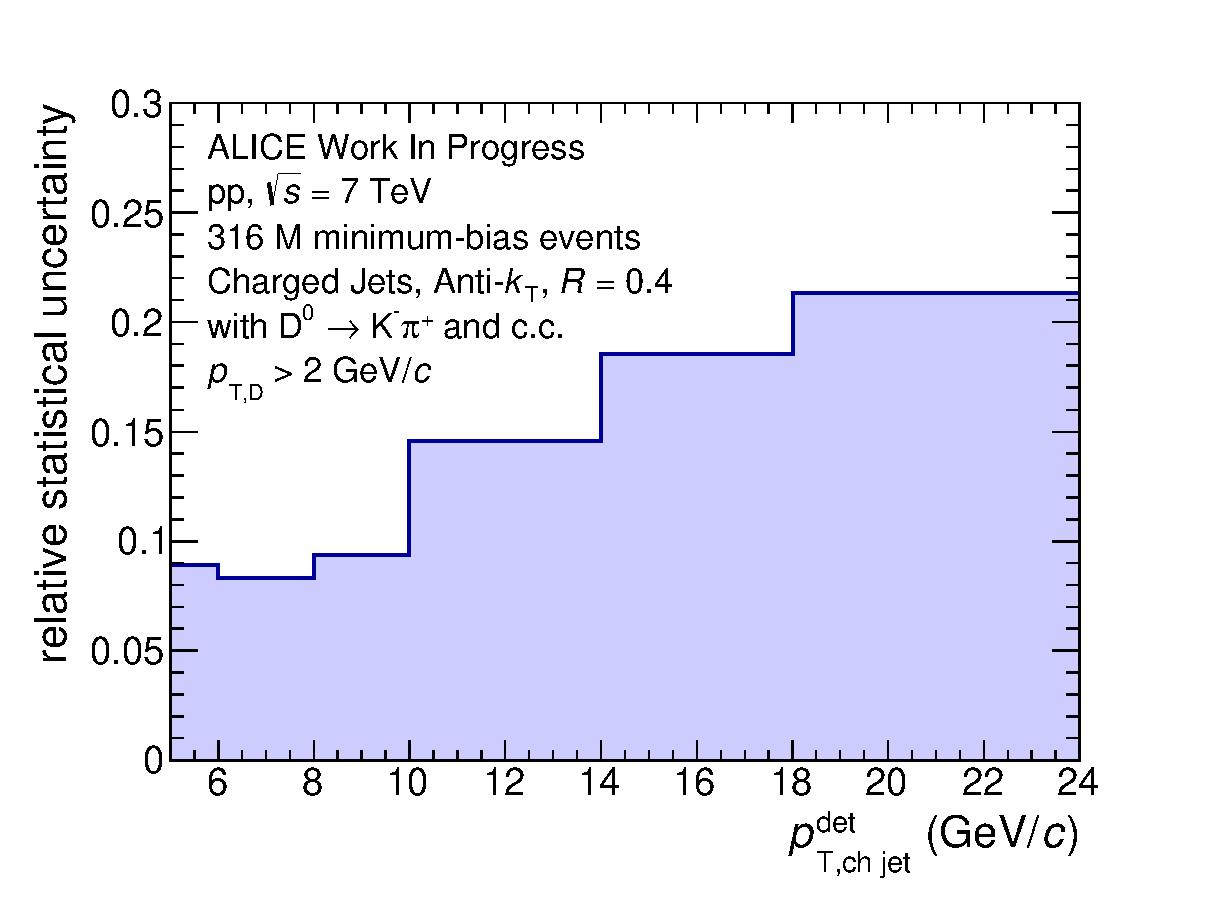
\includegraphics[width=\textwidth]{img/HQ16_WorkInProgress_StatisticalUncertainty} 
\column{.40\textwidth}
\begin{itemize}
\item Available statistics in 2010 (invariant mass fit method w/o efficiency correction)
\item Similar statistics as in MC simulation, but PYTHIA overestimates the signal/background
\end{itemize}
\end{columns}
\end{frame}

\begin{frame}{D-Tagged Jet Reconstruction Efficiency}
\begin{columns}
\column{.60\textwidth}
\begin{overpic}[width=\textwidth, trim=0 0 38 0, clip]{img/HQ16_Simulation_EfficiencyVsDPt}
\end{overpic}
\column{.40\textwidth}
\begin{itemize}
\item Dominated by \\ \textcolor{NavyBlue}{\Dzero\ reconstruction efficiency}
\item \alert{Strong increase with \ptd\ at low \ptd} \\
$\rightarrow$ topological cuts on the secondary vertex, tighter at low \ptd\
\end{itemize}
\end{columns}
\bigskip
\textcolor{ForestGreen}{No dependence on the \ptchjet}: simplifies corrections and reduces systematic uncertainties 
\end{frame}

\begin{frame}[t]{Jet Energy Scale shift and \pt\ resolution}
\begin{columns}
\column{.47\textwidth}
\begin{overpic}[width=\textwidth]{img/ALICE_JetRes}
\put (-3,4) {{\tiny PRD 91 (2015) 112012}}
\end{overpic}\\
\medskip
{\small
\textcolor{BrickRed}{
\textbf{Inclusive Charged Jets} \\
\medskip
$\mu [(\ptchjetdet-\ptchjetgen)/\ptchjetgen]\approx -3\%$ \\
\smallskip
$\sigma[(\ptchjetdet-\ptchjetgen)/\ptchjetgen]\approx17\%$
}}
\column{.53\textwidth}
\medskip
\begin{overpic}[width=\textwidth, trim=0 9 30 22, clip]{img/HQ16_Simulation_DetectorResponse}
\end{overpic}\\
\raggedleft
{\small
\textcolor{NavyBlue}{
\textbf{D-Tagged Charged Jets}\\
\medskip
$\mu[(\ptchjetdet-\ptchjetgen)/\ptchjetgen]\approx -3\%$ \\
\smallskip
$\sigma[(\ptchjetdet-\ptchjetgen)/\ptchjetgen]\approx11\%$
}}
\end{columns}
\bigskip
\centering
\textbf{slightly better \ptchjet\ resolution due to the D-meson requirement}
\end{frame}

\begin{frame}{JES shift and \pt\ resolution: \pt-dependence}
\begin{columns}
\column{.50\textwidth}
\centering
\textbf{JES shift}\\
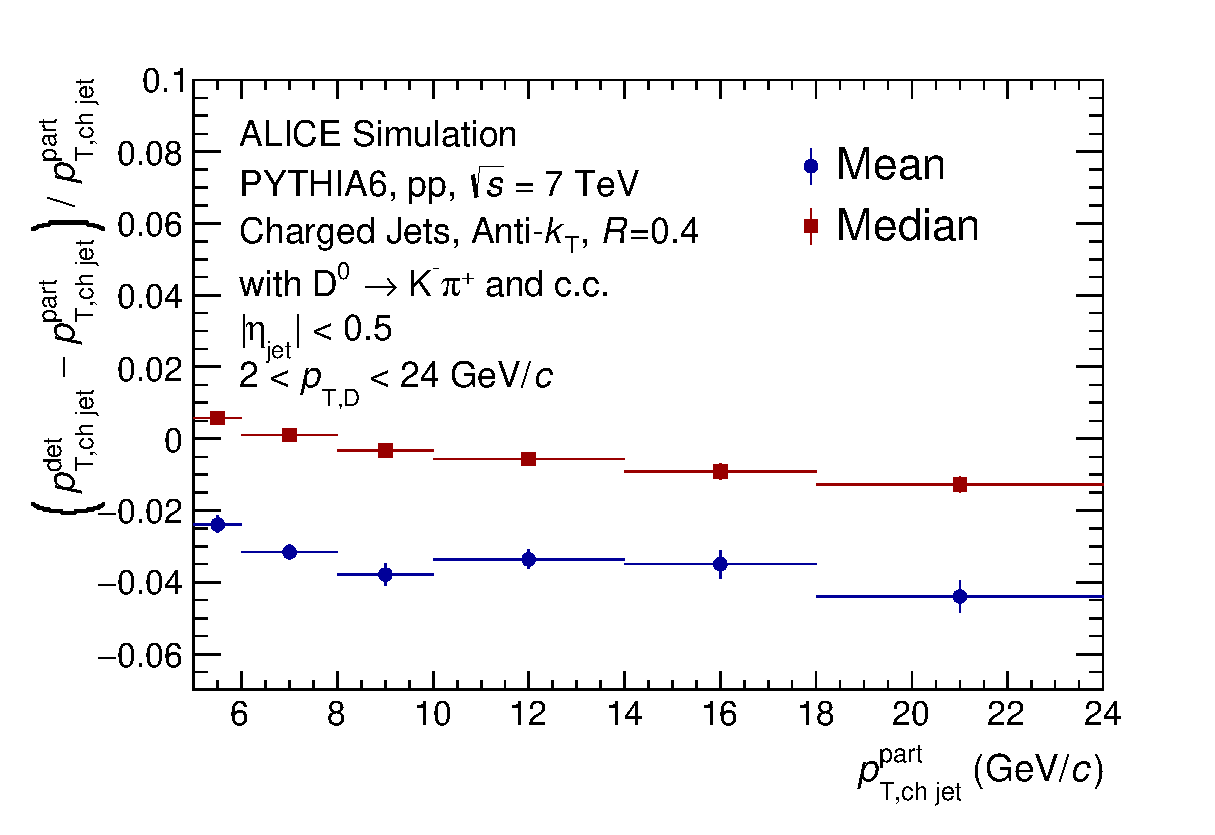
\includegraphics[width=\textwidth]{img/HQ16_Simulation_EnergyScaleShift}
\column{.50\textwidth}
\centering
\textbf{\ptchjet\ resolution} \\
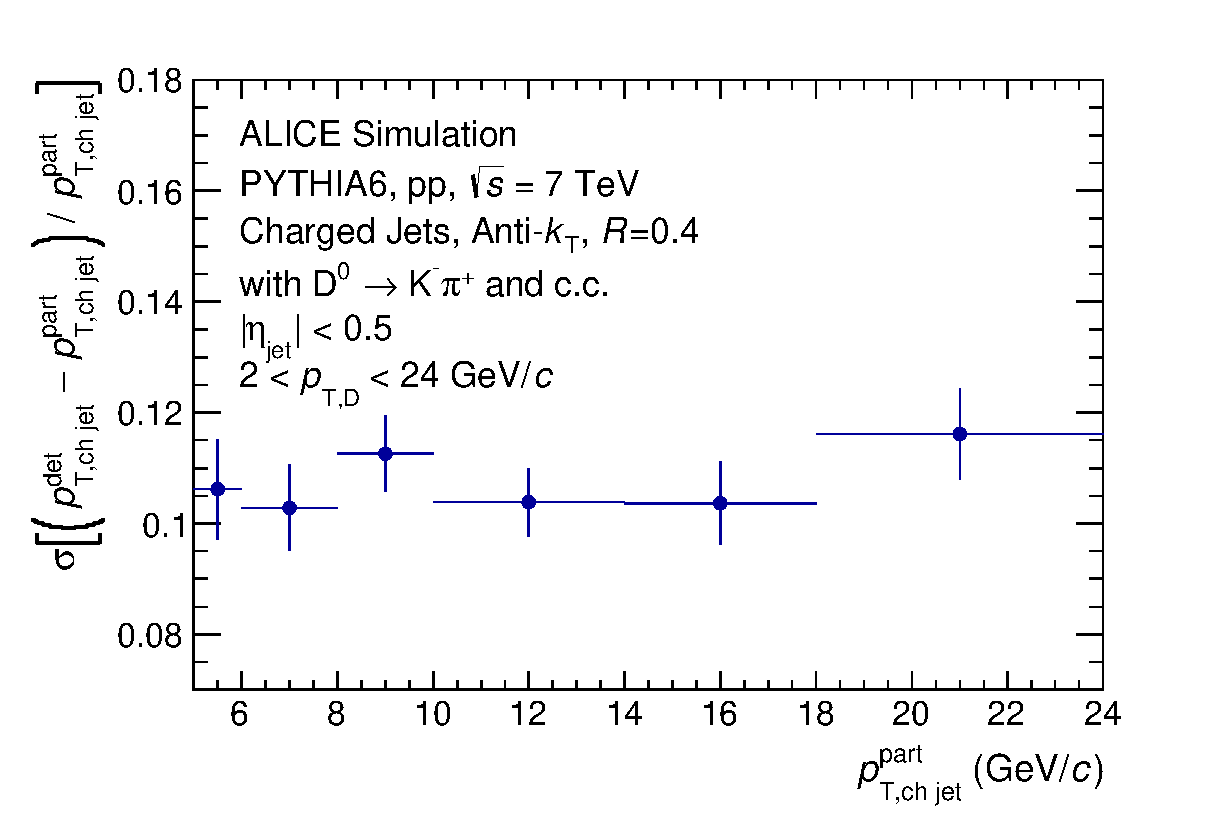
\includegraphics[width=\textwidth]{img/HQ16_Simulation_Resolution}
\end{columns}
\medskip
\begin{itemize}
\item JES shift and \ptchjet\ resolution dominated by \alert{tracking efficiency}
\item \alert{No significant \pt-dependence} in the range $5<\ptchjet<24$ \GeVc
\end{itemize}
\end{frame}

\end{document}
